\documentclass{standalone}
\usepackage{tikz}

\begin{document}

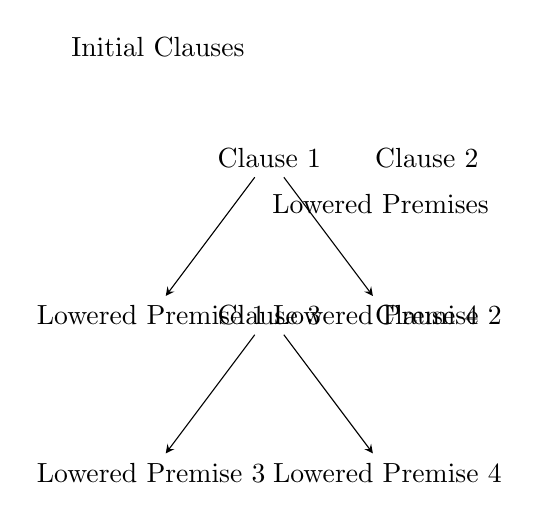
\begin{tikzpicture}[level distance=1.5cm,
                    level 1/.style={sibling distance=3cm},
                    level 2/.style={sibling distance=2cm},
                    level 3/.style={sibling distance=1.5cm},
                    node distance=2cm]

    % Nodes at level 1 (initial clauses)
    \node (C1) {Clause 1};
    \node (C2) [right of=C1] {Clause 2};
    \node (C3) [below of=C1] {Clause 3};
    \node (C4) [right of=C3] {Clause 4};

    % Nodes at level 2 (lowered premises)
    \node (L1) [below of=C1, xshift=-1.5cm] {Lowered Premise 1};
    \node (L2) [below of=C1, xshift=1.5cm] {Lowered Premise 2};
    \node (L3) [below of=C3, xshift=-1.5cm] {Lowered Premise 3};
    \node (L4) [below of=C3, xshift=1.5cm] {Lowered Premise 4};

    % Edges between nodes
    \draw[-stealth] (C1) -- (L1);
    \draw[-stealth] (C1) -- (L2);
    \draw[-stealth] (C3) -- (L3);
    \draw[-stealth] (C3) -- (L4);

    % Labels for clarity
    \node [above left of=C1] {Initial Clauses};
    \node [above right of=C3] {Lowered Premises};

\end{tikzpicture}

\end{document}